\documentclass[a4paper]{article}
\usepackage{graphicx} % para da cor
\usepackage[brazil]{babel} % Para traduzir nomes que aparecem em inglês na estrutura do documento.
\usepackage[utf8]{inputenc} % This package allows the user to specify an input encoding
\usepackage[T1]{fontenc} % Permite que o LaTeX compreenda a acentuação feita direto pelo teclado. 
\usepackage{amsfonts} % Define alguns estilos de letras para o ambiente matemático
\usepackage{fancyhdr} % Para fazer cabeçalhos personalizados
\usepackage{float}
\usepackage{hyperref} % Para tornar os links clicáveis
\hypersetup{
    colorlinks=true,
    linkcolor=blue,
    filecolor=blue,
    citecolor=blue,
    urlcolor=blue,
}
\usepackage{microtype} % evitando ligatures do tipo ff
\DisableLigatures{encoding = *, family = * }
\title{\textbf{Manifesto Hotmart 2.0}}
\author{Vitor Lopes \\ vitor.lopes@hotmart.com}
\begin{document}
\maketitle
\begin{abstract}
    A Hotmart é uma ótima empresa para se frequentar e se fazer amigos além de prover um excelente ambiente para integração e troca de conhecimento. Essas características são tão marcantes que estão presentes em seus pilares e mantras conforme descritos em seu código de conduta. Entretanto, no que diz respeito a processos e código legado, infelizmente temos muito a que melhorar.
    Este material tem como objetivo propor uma metodologia ágil e divertida para lidar com esses desafios.
\end{abstract}
\section{Introdução}
O termo sistema legado descreve um sistema antigo que permanece em operação em uma organização.[1] Geralmente utilizam bancos de dados obsoletos.\footnote{https://pt.wikipedia.org/wiki/Sistema\_legado}:
\begin{enumerate}
    \item dificuldade de compreensão das regras de negócio neles implementadas;
    \item desconhecimento das razões que levaram a determinadas decisões;
    \item problemas na estruturação dos módulos de código;
    \item miscelânea de estilos de programação;
    \item obsolescência das ferramentas de desenvolvimento;
    \item impossibilidade de reaproveitamento dos equipamentos nos quais são executados para execução de softwares mais atuais;
    \item Altos custos de manutenção;
    \item Software complexo;
    \item Software de suporte obsoleto;
    \item Hardware obsoleto;
    \item Sem conhecimento técnico;
    \item Negócio crítico;
    \item Backlog de solicitações de mudança;
    \item Documentação deficiente;
    \item Conhecimento empresarial incorporado;
    \item Mal compreendido pelos mantenedores;
\end{enumerate}

Ou seja, infelizmente a Hotmart está repleta de código legado e que nascem a cada dua mais. Para se ter uma ideia, veja a quantidade de repositórios que temos hoje no GitHub:

\begin{figure}[H]
    \centering
    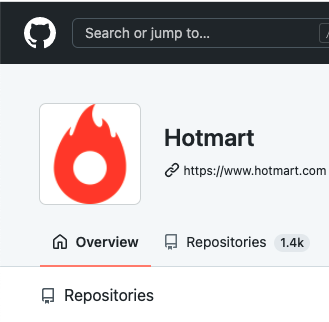
\includegraphics[scale=1,keepaspectratio=true]{images/01.png}
    \caption{Repositórios presentes no GitHub}
    \label{github_repo}
\end{figure}

Obviamente nem todos esses repositórios representam uma APP ou API, mas se formos conservadores e considerarmos 50\%, então teremos 700 repositórios onde nossas regras de negócio residem. Acho que levamos muito a sério a história de sair do monolito e acabamos criando tanto microserviço que as coisas podem ter saído um pouco do controle.

Mas então por que softwares legados existem? A resposta é simples: porque ninguém nasce sabendo aonde quer chegar. Uma empresa quando nasce, começa a ter que fazer suas escolhas. Ao longo do seu caminho, ela opta por boas ou não tão boas assim. Em um determinado momento, as escolhas passadas ajudam esta empresa a começar seguir em um caminho mais coeso. Isso se chama Maturidade.

\begin{figure}[H]
    \centering
    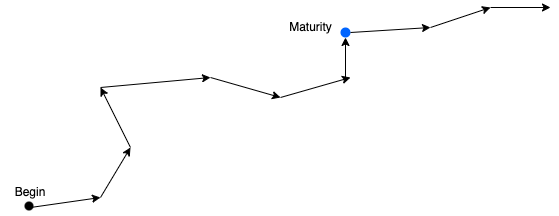
\includegraphics[scale=0.60,keepaspectratio=true]{images/02.png}
    \caption{Processo de amadurecimento}
    \label{mature_process}
\end{figure}

Se fosse possível pegarmos tudo de bom e ruim que trilhamos e juntar as melhores escolhas desde o momento em que nascemos até o momento em que amadurecemos, seria perfeito. E é exatamente o que é possível fazer com um software: a consolidação do conhecimento. 

\begin{figure}[H]
    \centering
    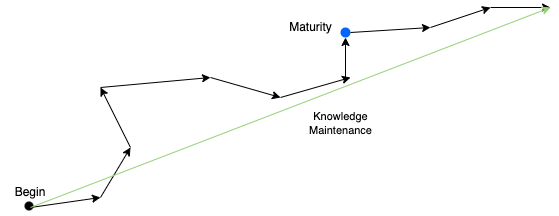
\includegraphics[scale=0.60,keepaspectratio=true]{images/03.png}
    \caption{Processo de consolidação do conhecimento}
    \label{knwledge_consolidation}
\end{figure}

Agora, mesmo que soubéssemos as melhores escolhas, de nada adiantaria chegar até aqui sem a correta manutenção de cada delas, ou seja, sendo que a cada nova decisão não fossem levadas em consideração todas as demais.

\begin{figure}[H]
    \centering
    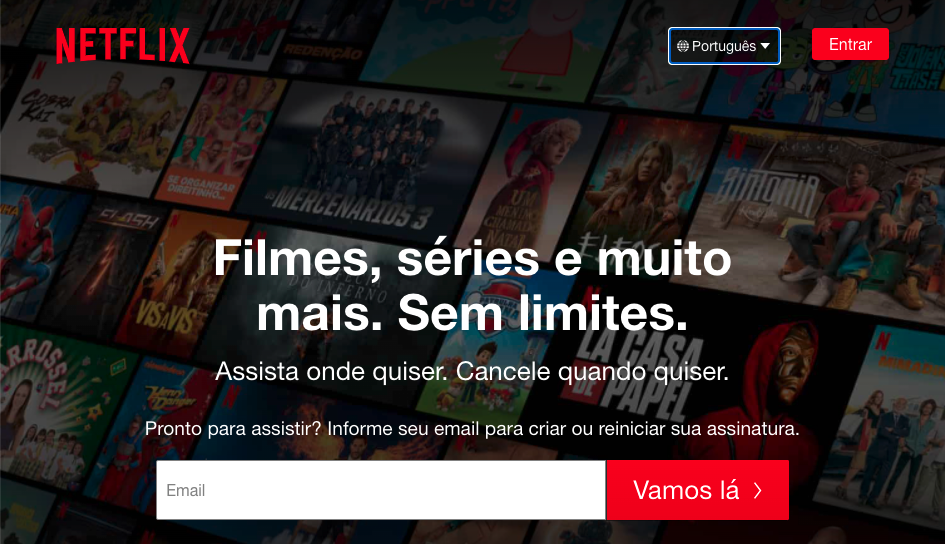
\includegraphics[scale=0.60,keepaspectratio=true]{images/04.png}
    \caption{Processo de manutenção do conhecimento}
    \label{knowledge_maintenance}
\end{figure}

Neste momento, estaríamos no que chamamos de ``Estado da Arte'' onde diversos setores da empresa poderiam trabalhar munidos de manuais para execução de seus trabalhos, deixando a parte criativa a ser utilizada no momento da criação de cada projeto. 

Em outras palavras, durante todo o processo de reconstrução do software e dos processos internos, os próprios times iriam criando sua cartilhas ou manuais de trabalho de modo que quando fosse necessário algum incremento ou atualização, todos os envolvidos já saberiam como agir tanto na demanda quanto na avaliação por pares \footnote{Pull Request, por exemplo}.

Mas se isso parece ser tão interessante, por quê nao se faz?

\section{Time em que está ganhando não se mexe}

Acredito que uma das respostas mais óbvias é a de que ``time em que está ganhando não se mexe’’. Mas e se Messi, Neymar, Cristiano Ronaldo tivessem iniciado a carreira em um time que estivesse ganhando, o que seriam deles?. EU advogo que todo processo deve ser revisto tantas vezes quantas forem necessários pois:
\begin{enumerate}
    \item você consegue melhorar o processo;
    \item você melhora a percepção que você tem do processo;
\end{enumerate}
Ou seja, sempre há uma melhora.

A análise e reconstrução leva tempo para se colher resultados, mas quando eles vêm, são muito significativos. Como uma amostra, há uma economia significativa de recursos computacionais e serviços de terceiros que poderíamos incorporar. Sem falar na redução drástica de tickets.

Não digo que a Hotmart nunca tenha feito mudanças nos códigos, mas clamo para que algum verdadeiramente profundo seja feito.

\section{O Monte Everest}

Outra frase muito ouvida é de que esse processo ou aquela informação é utilizada por tanta gente que me parece ser mais fácil Escalar o Monte Everest do que propor alguma mudança em meu contexto de trabalho.

\section{O Poder do Conhecimento}

Confesso que toda essa situação me deixava inquieto e após muita reflexão, tentei buscar na internet alguma resposta. Dentre o jargão corporativos norte-americano temos o padrão $C(x)O \; | \; x \in [A...Z]$ como por exemplo \emph{CEO}\footnote{Chief of Executive Officer}, \emph{CTO}\footnote{Chief of Technology Officer}, \emph{CFO}\footnote{Chief of Financial Officer} e tantos outros. 

Mas o que me chamou mais a atenção foi o \textbf{K}, da \textbf{CHIEF OF KNOWLEDGE OFFICER}. Dentre suas atribuições, temos\footnote{https://searchcio.techtarget.com/definition/CKO}:

\begin{quote}
    Chief knowledge officer (CKO) is a corporate title for the person responsible for overseeing knowledge management within an organization. The CKO position is related to, but broader than, the CIO position. The CKO's job is to ensure that the company profits from the effective use of knowledge resources. Investments in knowledge may include employees, processes and intellectual property; a CKO can help an organization maximize the return on investment (ROI) on those investments.
    Furthermore, a CKO can help an organization to:

    \begin{itemize}
        \item Maximize the return on investment (ROI) in knowledge.
        \item Maximize benefits from intangible assets, such as branding and customer relationships.
        \item Repeat successes and analyze and learn from failures.
        \item Promote best practices.
        \item Foster innovation.
        \item Avoid the loss of knowledge that can result from loss of personnel.
    \end{itemize}
\end{quote}

Portanto, o que temos hoje como um mantra talvez pudesse formar o quarto pilar: O Pilar do Conhecimento. E afinal de contas, é muito mais sustentar qualquer coisa com 4 pilares do que com apenas 3.

Duas outra característica bem interessante do Knowledge Officer são: 
\begin{itemize}
    \item Manter todo o conhecimento centralizado e organizado
    \item Extrair o que as pessoas têm de melhor a oferecer
\end{itemize}
Ou seja, esse Officer deve estar sempre de braços abertos a toda e qualquer iniciativa, dando acolhimento e direcionamento adequado. e o melhor de tudo, poderemos reescrever a missão da empresa, veja como:
\begin{quote}
    \textbf{EXTRAIR O QUE AS PESSOAS TÊM DE MELHOR A OFERECER PARA
    PERMITIR QUE AS PESSOAS POSSAM VIVER DE SUAS PAIXÕES}
\end{quote}

Isso seria excelência de ponta a ponta.

Para finalizar, para que tudo isso possa ser possível, seria necessária a criação de uma nova Torre, chamada de Torre do Conhecimento onde agregaria todos os Especialistas, Product Managers, Designers e Writers.
Essa Torre deveria receber as demandas da empresa, levantar requisitos, modelar entidades, elaboras layouts gráficos e textuais, e deve entregar um projeto no Jira já devidamente mensurado e organizado pronto para o time de desenvolvimento.

\section{Metodologia para Reconstrução de Processos}

Uma vez ouvi a seguinte frase dita por Gustavo Caetano\footnote{CEO da SambaTech} que nunca mais saiu de minha mente:
\begin{quote}
    \textbf{SE} você me traz um problema \\
    \textbf{MAS} não me traz a solução \\
    \textbf{ENTÃO} você faz parte do problema
\end{quote}

Depois de refletir por muito tempo, entendi que nem sempre sabemos a solução de todos os problemas assim quando nos deparamos com eles e que  todos devem ser reportados imediatamente para mitigar quaisquer efeitos negativos. Por isso, adaptei essa frase para algo um pouco mais tangível:
\begin{quote}
    \textbf{SE} você me traz um problema \\
    \textbf{ENTÃO} vamos discutir uma solução \\
    \textbf{POIS} juntos trabalhamos melhor
\end{quote}

Baseado nessa frase, gostaria de apresentar uma metodologia ágil que estou desenvolvendo para reconstrução de processos maduros a qual batizei de \textbf{AIOROS}. Por mais caricata ou incomum que pareça, esta metodologia foi baseada na série japonesa de mangá e anime chamada \textbf{Os Cavaleiros do Zodíaco} veiculada no Brasil por volta dos anos 90.

Apesar de possuir diversas sagas, a primeira nos interessa por fazer uma analogia quase perfeita para o contexto que precisamos, onde os cavaleiros de bronze precisam salvar a princesa ferida, correndo contra to tempo, e para isso precisam passar pelas 12 casas do zodíaco enfrentando seus guardiões.

\begin{figure}[H]
    \centering
    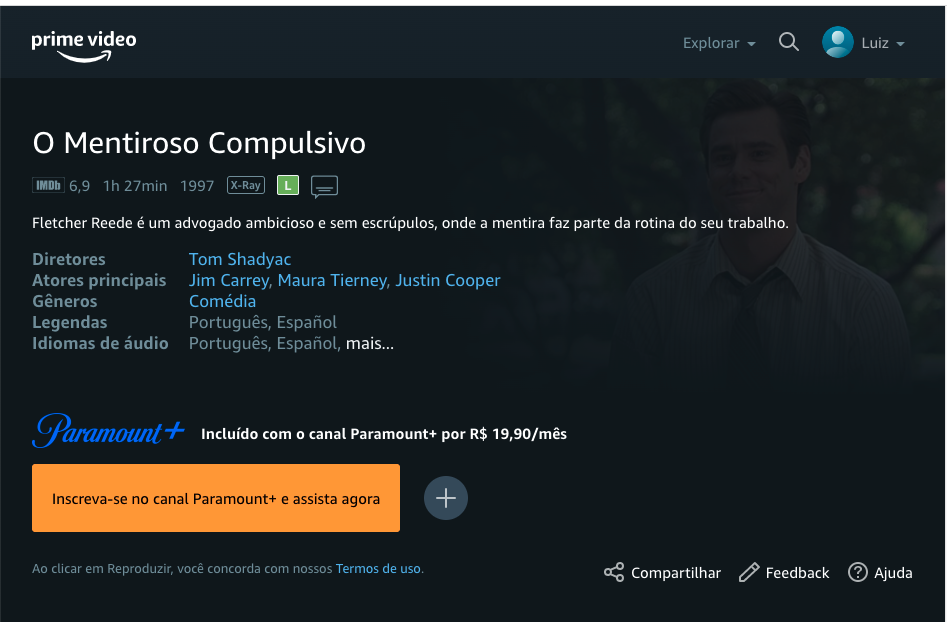
\includegraphics[scale=0.33,keepaspectratio=true]{images/06.png}
    \caption{Saori, reencarnação de Athena, ferida}
\end{figure}

Adaptando essa estória para nossa realidade, imagine que a princesa Saori seja a empresa ou o processo que está em execução de forma legada, ou seja, apenas com seu metabolismo basal não sendo capaz de entregar nada além do que suas funções básicas.

\begin{figure}[H]
    \centering
    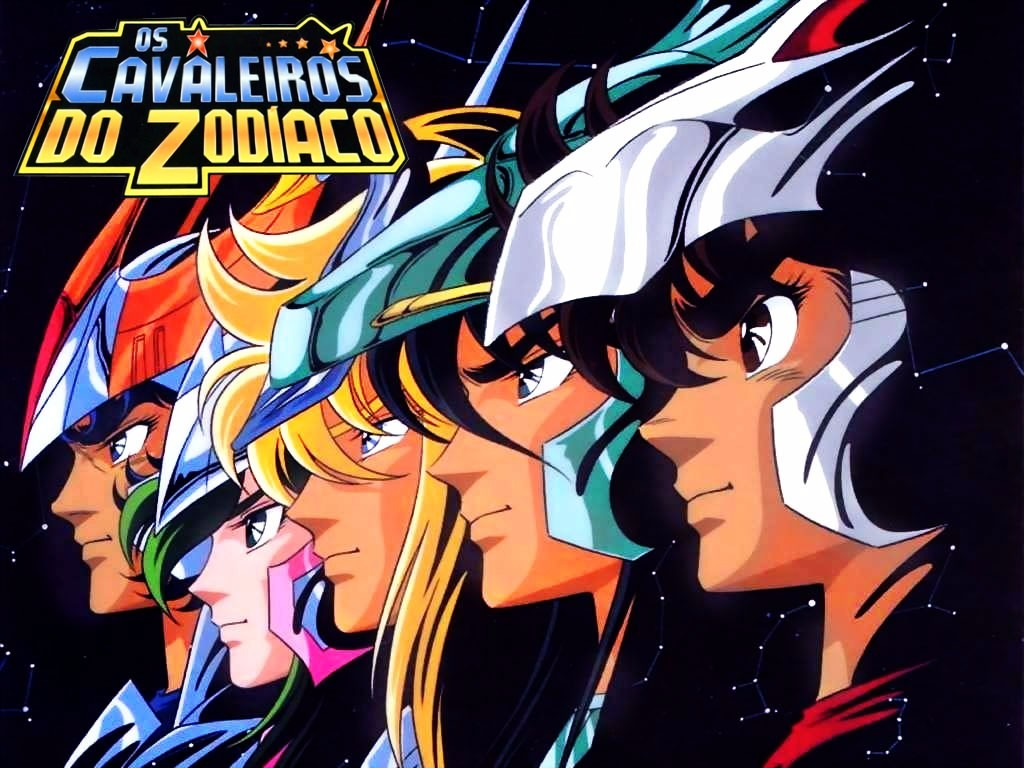
\includegraphics[scale=0.33,keepaspectratio=true]{images/05.jpg}
    \caption{Os Cavaleiros de Bronze}
\end{figure}

Já os cavaleiros de prata são os funcionários que reconhecem essa fraqueza nos processos legados e lutam arduamente em suas casas, enfrentando um guardião por vez.

\begin{figure}[H]
    \centering
    
\includegraphics[scale=0.35,keepaspectratio=true]{images/07.png}
    \caption{Relógio das 12 casas do Zodíaco}
\end{figure}

O Relógio do Zodíaco a agilidade, ou seja, o time não tem muito tempo a perder pois processos e clientes aguardam ansiosamente por melhorias e o time deve trabalhar de forma integrada, coesa, a fim de garantir entregar dentro do prazo.

\begin{figure}[H]
    \centering
    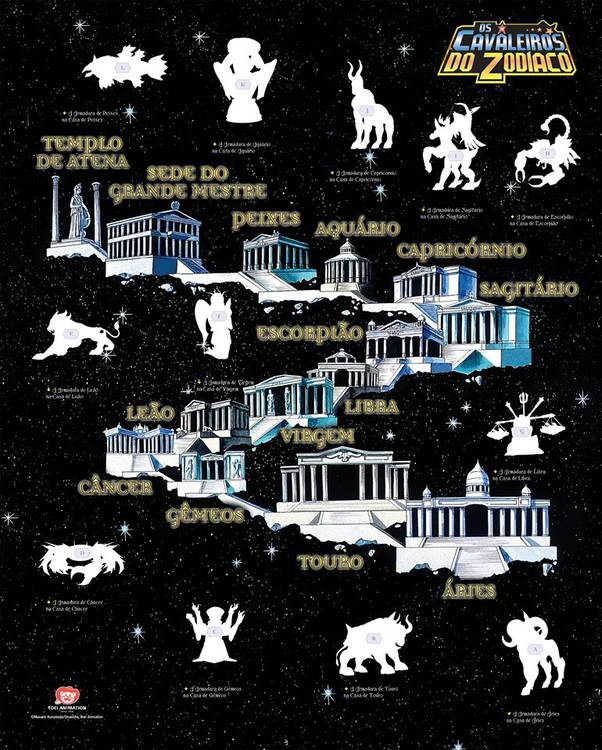
\includegraphics[scale=0.55,keepaspectratio=true]{images/08.jpg}
    \caption{As 12 casas do Zodíaco}
\end{figure}

As 12 Casas do Zodíaco representam em quantas partes o processo como um todo deverá ser quebrado. Deste ponto de vista, faz mais sentido dizer \textbf{As \emph{n} Casas do Zodíaco}. Mas aqui vale uma ressalva: 
\begin{itemize}
    \item Poucas casas deixam o sistema muito coeso, de difícil manutenção e com Cavaleiros de mais para combater
    \item Muitas casas deixar o sistema muito esparso, de difícil manutenção e com Cavaleiros de menos para combater
\end{itemize}

O segredo é ter uma equipe experiente para se definir qual é o número ideal de casas.

Portanto, vamos ver como isso funcionaria na prática
\begin{enumerate}
    \item Em uma reunião inicial a fim de explicar a todos os interessados o que será feito daqui pra frente;
    \item Em uma segunda reunião, de preferência com os membros mais experientes, deve-se de definir quais serão as casas a serem atacadas bem como nomear seus guardiões\footnote{deve-se haver pelo menos 2 guardiões para que haja uma cooperação mútua}
    \item Os guardiões, de posse de suas casas, devem definir os critérios de aceite e as regras de negócio que acharem pertinente à sua casa.
    \item Agora é a vez dos cavaleiros utilizarem do que há de melhor, elevando seus cosmos ao sétimo sentido, propondo soluções engenhosas que capazes de cobrir tudo que foi proposto pelos guardiões daquela casa. 
    \item Neste momento, Product Managers, Designers e Writers atuam ativamente na composição da solução do produto.
    \item Estes passos devem ser repetidos até que todo o projeto tenha finalizado. 
    \item Agora, Product Managers, Designers e Writers devem dar um formato no projeto, adicionando Epic, Estória, Tarefa, Sub-Tarefa para que os times executantes possam indicar o esforço para cada tarefa descrita. 
    \item Writers, não se esqueçam de que faz parte da entrega todas as chaves estarem traduzidas quando o projeto estiver fechado, ou seja, o time de desenvolvimento não poderá iniciar qualquer tarefa desde que essa condição não seja satisfeita. Essa entrega pode ser feita até via arquivo de texto anexado no card do jira, por exemplo.
    \item Voltando a falar sobre mensurar, como já teremos nosso livro de referência, teremos uma grande noção do quanto dura cada atividade, pelo menos uma boa aproximação. Dessa forma, fica bem mais simples e preciso saber quando uma tarefa deverá ser finalizada.
\end{enumerate}

% \section{A Inovação}

% Uma vez em que estivermos rodando os nossos trabalhos no ``Estado de arte'', sobrará muito tempo livro para criarmos e inovamos. 

% Por exemplo, imagine se a Hotmart fosse da seguinte maneira:
% % \begin{figure}[H]
% %     \centering
% %     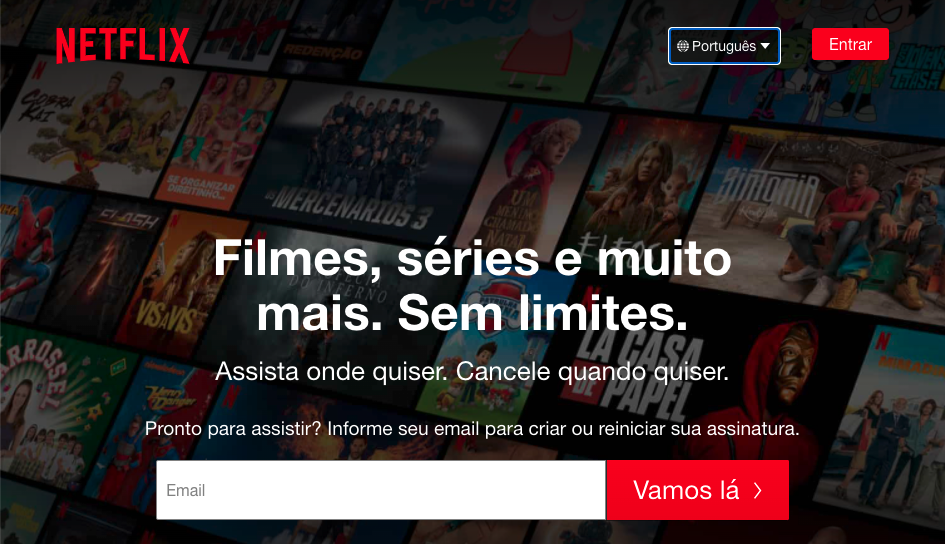
\includegraphics[scale=0.37,keepaspectratio=true]{images/04.png}
% %     \caption{Tela de login independente de haver compras}
% % \end{figure}

% % \begin{figure}[H]
% %     \centering
% %     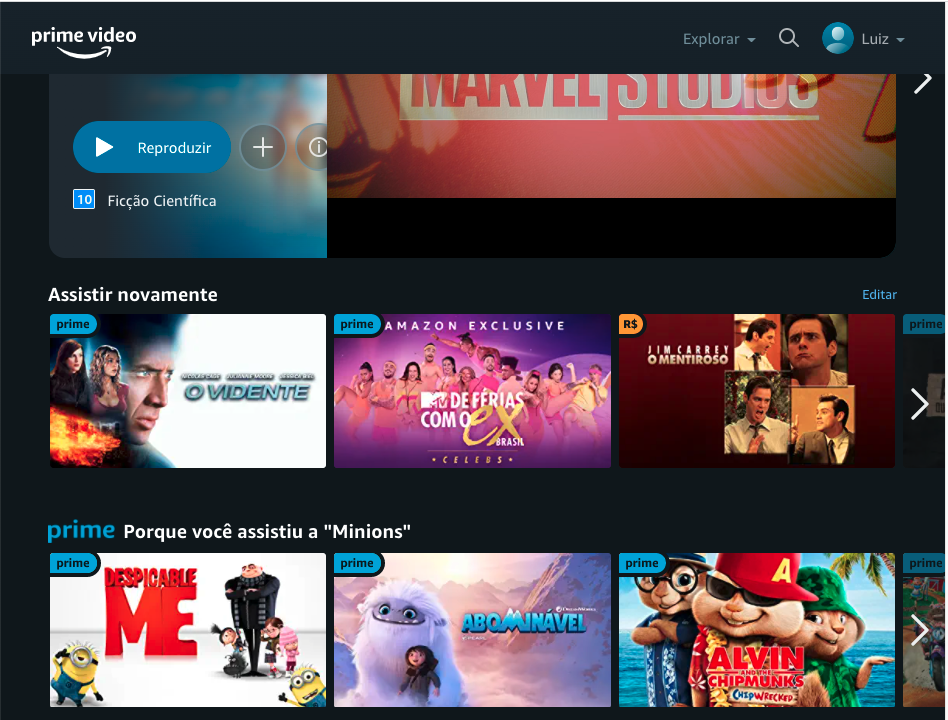
\includegraphics[scale=0.30,keepaspectratio=true]{images/05.png}
% %     \caption{Novidades do catálogo Hotmart, conteúdo gratuito oferecido pelo produtor como um trailer de seu produto}
% % \end{figure}

% % \begin{figure}[H]
% %     \centering
% %     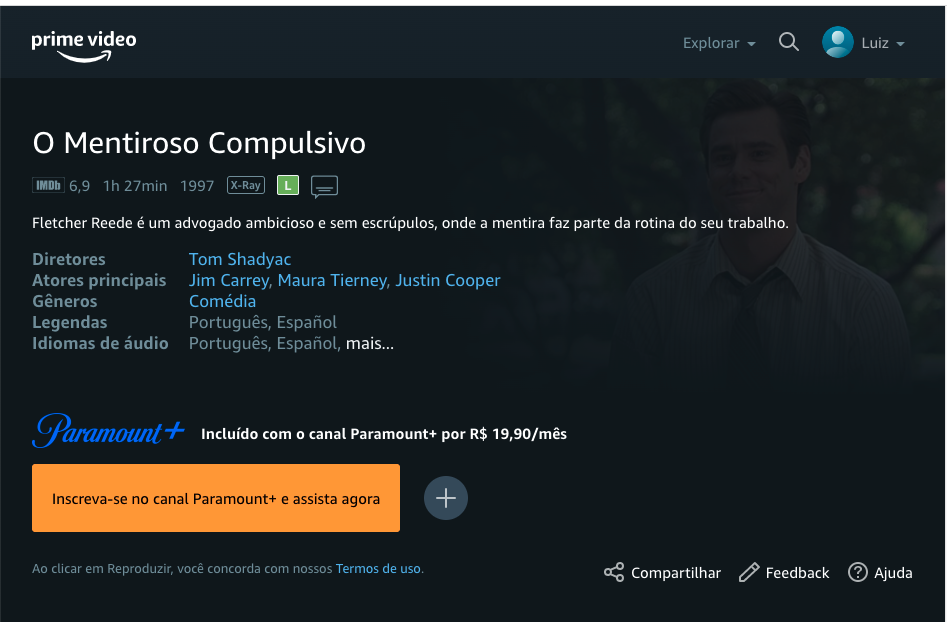
\includegraphics[scale=0.40,keepaspectratio=true]{images/06.png}
% %     \caption{Página de vendas de um pequeno, médio ou grande produtor}
% % \end{figure}

% % \begin{figure}[H]
% %     \centering
% %     
\includegraphics[scale=0.50,keepaspectratio=true]{images/07.png}
% %     \caption{Tela superior deve conter: COMPRAR - MINHAS COMPRAS - VENDER - MINHAS VENDAS - AJUDA}
% % \end{figure}

% \section{Conclusão}

% Acredita-se que se a plataforma por voltada para o comprador, conseguiremos melhores performances justamente pelo efeito orgânico da internet. A ideia é posicionar a Plataforma onde YouTube, Amazon Prime e Netflix não posicionaram. Seria ficar ali no meio deles servindo o que eles não servem. 

% Imagine ver aquela gameplay completinha do seu gamer favorito pagando 3,99 sem anúncio? e ainda ter uma porrada de funcionalidade exclusiva. Seria muito melhor, pelo menos eu acho. E eles têm muitas dores com o YouTube onde sao cancelados por direitos autorais. Na nossa plataforma, ele poderia colocar uma música do Pink Floyd se quisesse desde que recolhesse os direitos aos autores. Seria um modelo onde todo mundo ganha.

% Poderíamos aplicar o reembolso que nem na Steam: jogou por mais de 2 horas, sem reembolso. Isso iria reduzir bastante demanda de suporte e ticket pra gente. 

% Fora que poderíamos fazer parcerias com as universidades para aprimorar nossos algoritmos de classificação, clusterização e sistema de busca e recomendação. 

\end{document}